\documentclass[14pt,a4paper]{extreport}

\usepackage[utf8]{inputenc}
\usepackage[romanian]{babel}

% \renewcommand\familydefault{\sfdefault} % computer modern sans serif
\usepackage{fontspec}
\setmainfont{Times New Roman}


\linespread{1}

\usepackage{geometry}
 \geometry{
 left=20mm,
 right=10mm,
 top=20mm,
 bottom=20mm,
 % showframe
}

\usepackage{xcolor}
\definecolor{mygreen}{rgb}{0,0.6,0}
\definecolor{mygray}{rgb}{0.5,0.5,0.5}
\definecolor{mymauve}{rgb}{0.58,0,0.82}
\definecolor{darkgray}{rgb}{.4,.4,.4}
\definecolor{navy}{HTML}{000080}
\definecolor{purple}{rgb}{0.65, 0.12, 0.82}
\definecolor{codepurple}{rgb}{0.58,0,0.82}
\definecolor{backcolour}{rgb}{0.95,0.95,0.92}

% Please add the following required packages to your document preamble:
\usepackage{multirow}
\usepackage{array}

\usepackage{caption}
% \usepackage[singlelinecheck=false]{caption}

% \captionsetup[table]{name=Tabelul}

\usepackage{graphicx}
\graphicspath{ {fig} }

\usepackage{amsmath} % for the equation* environment

\usepackage{xcolor}   % for \textcolor
\usepackage{listings}
\lstset{
  columns=fullflexible,
  frame=single,
  breaklines=true,
  postbreak=\mbox{\textcolor{red}{$\hookrightarrow$}\space},
}
\usepackage{csvsimple}

\begin{document}

\begin{titlepage}
\begin{center}
	{\large{ Universitatea Tehnica a Moldovei \\}}
	{\large{ Facultatea Calculatoare, Informatică și Microelectronică \\}}
	{\large{ Departamentul Ingineria Software și Automatică \\}}
	\vspace{4cm}
	{\LARGE {\bf{ Raport }}}\\
	\vspace{1cm}
	{\large { Lucrarea de Laborator Nr.3 \\}}
	{\large { Analiza și Proiectarea Algoritmilor \\}}
	{\large { Tema: Algoritmi greedy  \\}}
\end{center}

\vspace{5cm}

\noindent{\large A efectuat:\hfill St. gr. TI-206} \\
\noindent{\large\null\hfill Pleșu Cătălin} \\
\noindent{\null} \\
\noindent{\large A verificat:\hfill Lect. Univ.} \\
\noindent{\large\null\hfill Bîtca Ernest} \\

\vspace{5cm}

\centering{\large{ Chișinău 2021 }}
\end{titlepage}


\clearpage
\subsection*{Scopul:\\}
\begin{enumerate}
	\item Studierea tehnicii greedy. 
	\item Analiza şi implementarea algoritmilor greedy. 
\end{enumerate}

\subsection*{Sarcina:}
\begin{enumerate}
	\item De studiat tehnica greedy de proiectare a algoritmilor. 
	\item De implementat într-un limbaj de programare algoritmii Prim şi Kruskal. 
	\item De făcut analiza empirică a algoritmilor Kruskal şi Prim. 
	\item De alcătuit un raport. 
\end{enumerate}
 
\clearpage
\subsection*{ Întrebări de control: \\}
\begin{enumerate}
	\item Descrieţi metoda greedy. 
	\item Când se aplică algoritmul Kruskal şi când algoritmul Prim ? 
	\item Ce tip de date este comod de folosit la elaborarea programului al unui algoritm de tip greedy? 
	\item Care sunt avantajele şi dezavantajele algoritmilor Prim si Kruskal?
\end{enumerate}

\begin{enumerate}
	\item{Algoritmii greedy (greedy = lacom) sunt în general simpli şi   
sunt folosiţi la rezolvarea problemelor de optimizare, cum ar fi: să   
se găsească cea mai bună ordine de executare a unor lucrări pe 
calculator, să   se găsească cel mai scurt drum într-un graf etc. În 
cele mai multe situaţii de acest fel avem: 
	\begin{itemize}
		\item  mulţime de candidaţi (lucrări de executat, vârfuri ale grafului etc); 
		\item o funcţie care verifică dacă o anumită mulţime de candidaţi constituie o soluţie posibilă, nu neapărat optimă, a problemei; 
		\item o  funcţie  care verifică dacă o mulţime de candidaţi este fezabilă, adică dacă este posibil să   completăm această mulţime astfel încât să   obţinem o soluţie posibilă, nu neapărat optimă, a problemei; 
		\item o  funcţie  de selecţie care indică la orice moment care este cel mai promiţător dintre candidaţii încă nefolosiţi;
		\item o  funcţie  obiectiv care dă valoarea unei soluţii (timpul necesar executării tuturor lucrărilor într-o anumită ordine, lungimea drumului pe care l-am găsit etc); aceasta este funcţia pe care urmărim să   o optimizăm (minimizăm/maximizăm). 

	\end{itemize}
Pentru a rezolva problema de optimizare, se caută o soluţie 
posibilă care să   optimizeze valoarea  funcţiei obiectiv. Un algoritm 
greedy construieşte soluţia pas cu pas.
Iniţial, mulţimea candidaţilor 
selectaţi este vidă. La fiecare pas, se   adaugă acestei mulţimi cel 
		}
	\item Algoritmul Kruskal se aplică atunci când avem un număr mare de noduri dar un numări mic de muchii și totodată muchiile sunt ordonate și nu este nevoie să le sortăm. 
Algoritmul Prim se aplică atunci când avem un număr mare de muchii unde algoritmul Kruskal s-ar descurca mai rău.

\item La elaborarea programului pentru algoritmii greedy este comod de utilizat arbori, stive și cozi. Totodată s-ar fi putut utiliza și un dictionar sau hash.

\item Avantajul algoritmului Prim este că se execută bine atunci când numărul de vârfuri este mic. Avantajul algoritmului Kruskal este că se execută bine atunci când numărul de muchii este mic. 
\end{enumerate}

\clearpage
\subsection*{Testarea empirică a algoritmilor}
%cazul 1
\subsection*{}{
\begin{table}[h]
\captionsetup{singlelinecheck = false, justification=raggedright}
	\caption{Timpul de rulare, puține vârfuri}
\label{tab:rulare_min} 
\begin{center}
	\csvautotabular{../data.csv}
\end{center}
\end{table}
\paragraph{}
\begin{figure}[h]
\begin{center}
	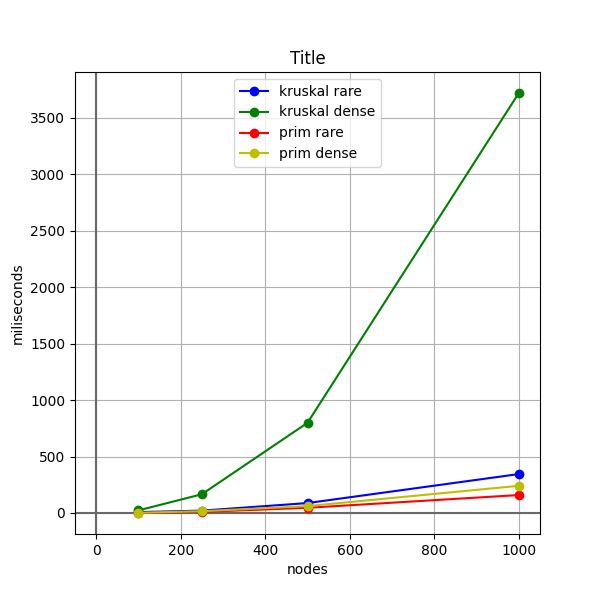
\includegraphics[width=12cm]{data_min}
	\caption{Timpul de rulare din tabela ~\ref{tab:rulare_min}} 
	\label{fig:rulare_min} 
\end{center}
\end{figure}
\paragraph{}
După cum se observă în Figura ~\ref{fig:rulare_min} atunci când avem un număr mai mare de muchii în arbore indiferent de algoritm, arborele de acoperire minim va fi găsit mai greu. Totodată observăm că atunci când arborele este dens algoritmul Kruskal se comportă rău. Analizând doar această imagine ne putem gândi că algoritmul Prim va fi mai eficient pentru toate cazurile.
}
%cazul 2
\subsection*{}{
\begin{table}[h]
\captionsetup{singlelinecheck = false, justification=raggedright}
	\caption{Timpul de rulare, 20000 vârfuri}
	\label{tab:rulare_max} 
\begin{center}
	\csvautotabular{../data_max.csv}
\end{center}
\end{table}
\paragraph{}
\begin{figure}[h]
\begin{center}
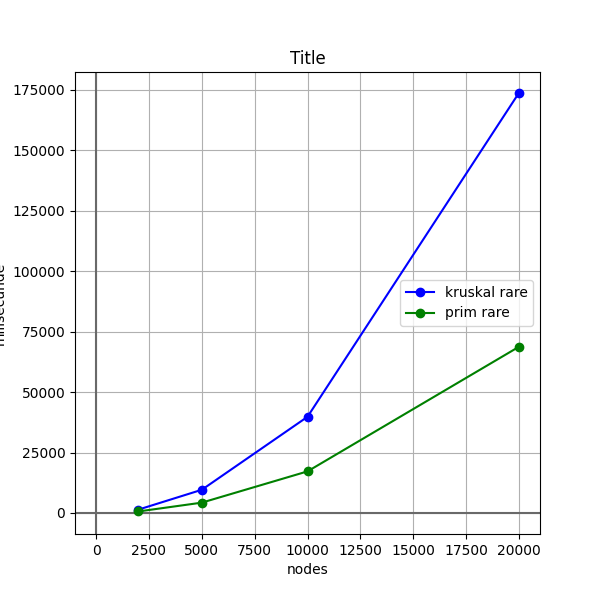
\includegraphics[width=12cm]{data_max}
	\caption{Timpul de rulare din tabela ~\ref{tab:rulare_max}} 
	\label{fig:rulare_max} 
\end{center}
\end{figure}
\paragraph{}
După cum se observă în Figura ~\ref{fig:rulare_max} algoritmul prim rămâne a fi mai eficient decât algoritmul lui kruskal și pentru un număr mai mare de vârfuri, până la 20000.
}
%cazul 3
\subsection*{} {
\begin{table}[h]
\captionsetup{singlelinecheck = false, justification=raggedright}
	\caption{Timpul de rulare, 35000 vârfuri}
	\label{tab:rulare_mega} 
\begin{center}
	\csvautotabular{../data_mega.csv}
\end{center}
\end{table}
\paragraph{}
\begin{figure}[h]
\begin{center}
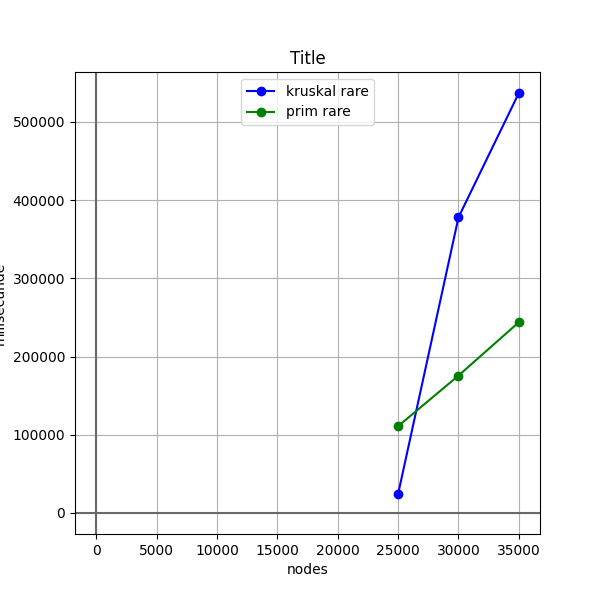
\includegraphics[width=13cm]{data_mega}
	\caption{Timpul de rulare din tabela ~\ref{tab:rulare_mega}} 
	\label{fig:rulare_mega} 
\end{center}
\end{figure}
\paragraph{}
În experimentul din tabela ~\ref{tab:rulare_mega} am încercat să demonstrez că, când numărul de vârfuri este mai mare algoritmul prim va fi se mai ineficient decât algortmul kruskal, sau cel puțin să arăt că valoarea lui prim se apropie incet de kruskal, însă nu s-a primit să demonstrez acest lucru cu datele care le am la dispoziție.
}

\clearpage
\subsection*{Testarea programului}
\paragraph{}
Pentru a testa corectitudinea programului voi genera un graf rar de 10 elemente, voi rezolva afla arborele de acoperire minim cu ajutorul unui algoritm oarecare de mână, apoi voi rula programul asupra acestui graf pentru a compara rezultatele.

\begin{figure}[h]
\begin{center}
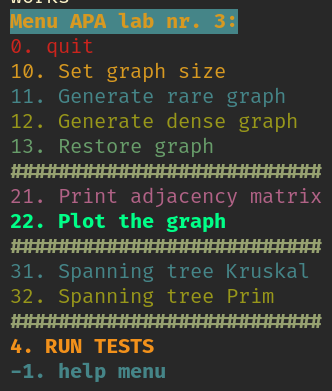
\includegraphics[width=10cm]{menu}
	\caption{Meniul programului} 
	\label{fig:menu} 
\end{center}
\end{figure}

\begin{figure}[h]
\begin{center}
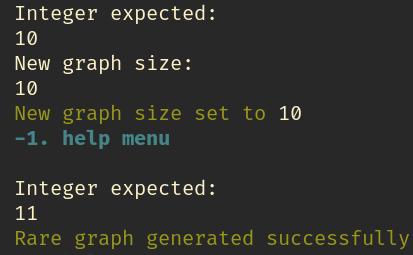
\includegraphics[width=10cm]{new_graph}
	\caption{Generarea unui graph rar} 
\end{center}
\end{figure}

\begin{figure}[h]
\begin{center}
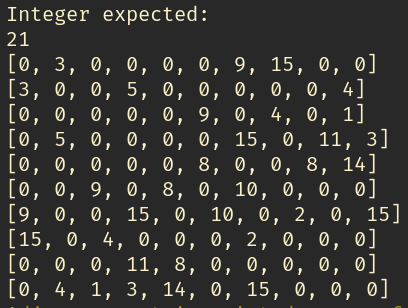
\includegraphics[width=10cm]{adjacency}
	\caption{Matricea de adiacență} 
\end{center}
\end{figure}

\begin{figure}[h]
\begin{center}
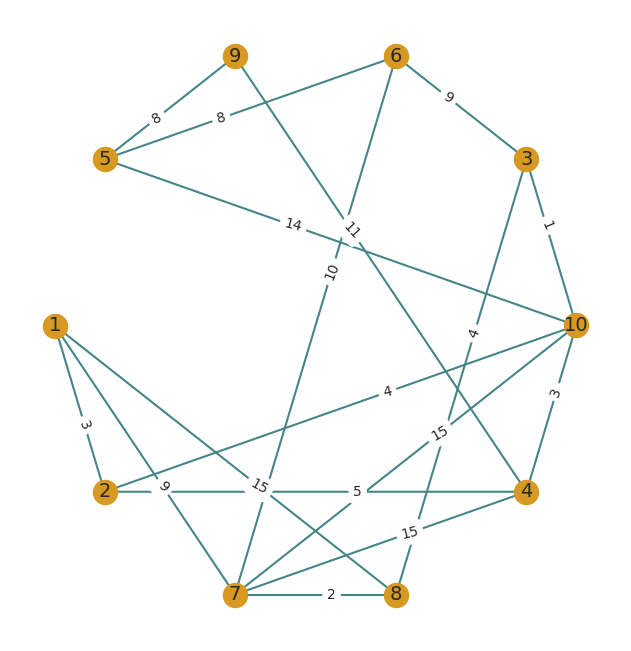
\includegraphics[width=15cm]{graph}
	\caption{Graful generat} 
\end{center}
\end{figure}

\begin{figure}[h]
\begin{center}
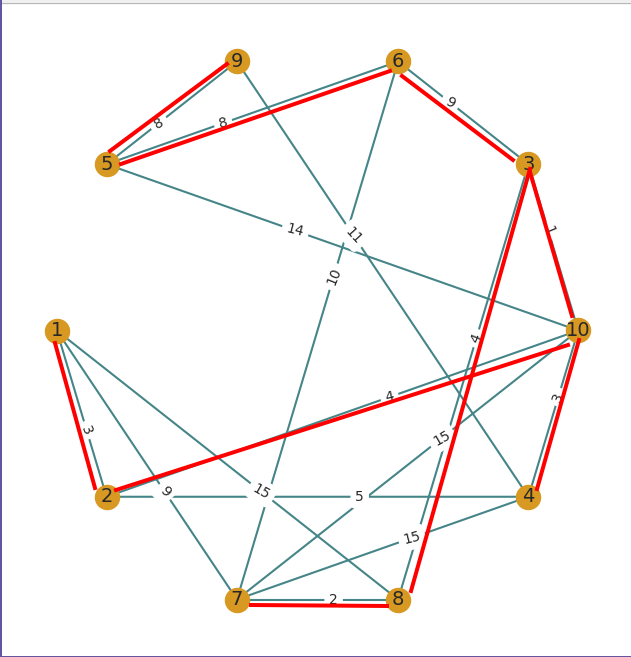
\includegraphics[width=15cm]{arbore_min}
	\caption{Arborele de acoperire identificat manual} 
\end{center}
\end{figure}

\begin{figure}[h]
\begin{center}
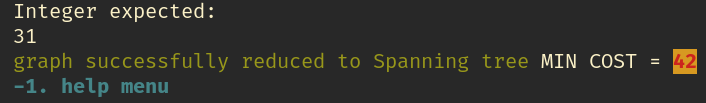
\includegraphics[width=15cm]{kruskal}
	\caption{Generarea arborelui de acoperire minim prin metoda Kruskal} 
\end{center}
\end{figure}

\begin{figure}[h]
\begin{center}
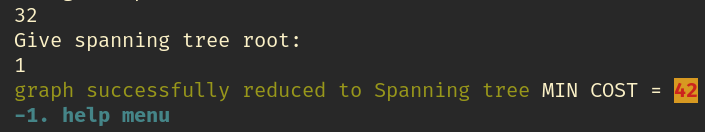
\includegraphics[width=15cm]{prim}
	\caption{Generarea arborelui de acoperire minim prin metoda Prim} 
\end{center}
\end{figure}

\begin{figure}[h]
\begin{center}
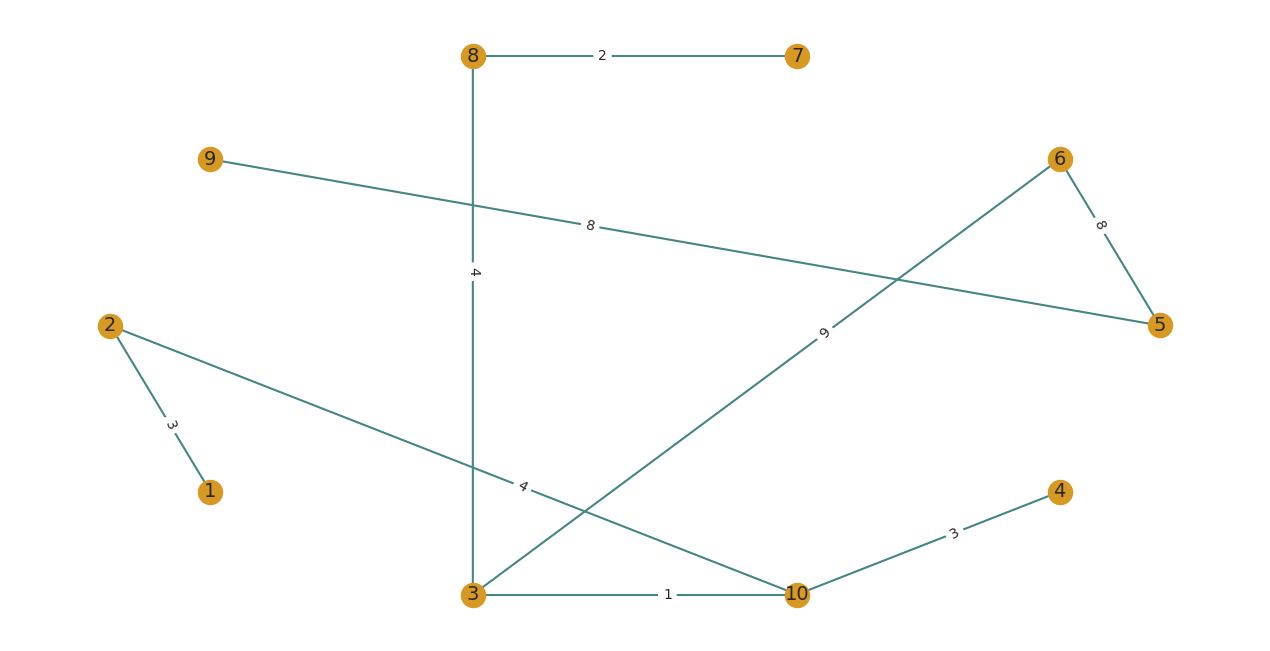
\includegraphics[width=18cm]{acoperire}
	\caption{Arborele de acoperire calculat prin ambele metode} 
\end{center}
\end{figure}

\clearpage
\subsection*{Concluzii:}
\paragraph{}
În cadrul acestei lucrări de laborator am învățat depre algoritmii greedy si anume mi-am adus aminte algoritmul lui Kruskal și Prim.
\paragraph{}
Comparând arborii calculați de calculator și arborele gasit de mine am stabilit că algoritmii au fost implementați corect.
\paragraph{}
Am comparat acești algoritmi pe cale empirică.Rezultatele obținute ne arată că în toate cazurile algoritmul Prim va fi mai eficient decât algoritmul Kruskal. 

\vfill
\begin{flushright}
\LaTeX
\end{flushright}


\appendix
\clearpage
\section*{Anexa main.rs}
\lstinputlisting[frame=none]{../src/main.rs}

\clearpage
\section*{Anexa kruskal.rs}
\lstinputlisting[frame=none]{../src/kruskal.rs}

\clearpage
\section*{Anexa prim.rs}
\lstinputlisting[frame=none]{../src/prim.rs}

\clearpage
\section*{Anexa main.py}
\lstinputlisting[frame=none]{../src/main.py}

\end{document}
